%=====================================================
%====== If you are new to LaTeX, this website ========
%======     will be your new best friend:     ========
%======   http://en.wikibooks.org/wiki/LaTeX  ========
%======   Template created by Jonathan Blair  ========
%=====================================================



%=====================================================
%============ Controls ===============================
%=====================================================

%\documentclass[12pt,letterpaper,onecolumn]{article}
\documentclass[11pt,letterpaper,onecolumn]{article}
%\documentclass[10pt,letterpaper,onecolumn]{article}  % not recommended
%\documentclass[12pt,letterpaper,twocolumn]{article}
%\documentclass[11pt,letterpaper,twocolumn]{article}
%\documentclass[10pt,letterpaper,twocolumn]{article}


\usepackage{amsmath}
\usepackage{graphicx}
\usepackage{url}
\usepackage{textgreek}
\usepackage{float}
\usepackage{booktabs}
%\graphicspath{{path-to-folder-containing-necessary-graphics}{other folder as necessary}}


%=====================================================
%============ \begin{document} =======================
%=====================================================

\begin{document}

%=====================================================
%============ Title ==================================
%=====================================================

\title{\bf RLC Circuits and Resonant Behavior}
%\title{\Large\bf Larger, Bolded Title}

%=====================================================
%============ Author =================================
%=====================================================
\author{
 Jairo Portillo \\*
  \\*
 PHY 338K Electronic Techniques \\*
 Department of Physics \\*
 The University of Texas at Austin \\*
 Austin, TX 78712, USA
}
\date{February 10, 2016}

%\address{The University of Texas, Austin, Texas, 78712}

\maketitle

%=====================================================
%============ Abstract ===============================
%=====================================================

\begin{abstract}

In this lab, we were to become acquainted with a RLC circuit and a trap filter RLC circuit. We observed and measured the behavior of the input and output voltages, then plotting the transfer function for both configurations. We are able to model the behavior of the circuits and find for out configurations that the resonant frequency is at 129.949 kHz.     
\end{abstract}

%=====================================================
%============ Body of the article ==========================
%=====================================================

%=====================================================
%============ Section ==================================
%=====================================================

\section{Preperation}

In preparation for this lab, we has to review phasor diagrams and AC circuit analysis. We also derived the transfer functions for both configurations of the RLC circuit. Using Kirchhoff's laws and the impedance of capacitors and inductors, we can find the transfer function. We simply use the relation 
$$T(\omega) = \frac{V_{out}}{V_{in}}=\frac{Z_{out}}{Z_{in}+Z_{out}}$$
where $Z_{out}$ is the impedance for the output voltage and $V_{in}$ is the impedance for the input voltage. For the series RLC, the transfer function can be found with 
$$T(\omega)=\frac{Z_C}{Z_C+R}=\frac{R}{R+\frac{1}{j\omega C}+j\omega L}$$
with much algebra it can be simplified to
$$T(\omega) = \frac{R}{\sqrt{R^2 + \omega^2L^2 + \frac{1}{\omega^2C^2}-\frac{2L}{C}}}$$
where R is the resistance, C is the capacitance, L is the inductance, and $\omega$ is the frequency. For the notch/trap circuit, we find the tranfer function to be
$$T(\omega)=\frac{j\omega L+\frac{1}{j\omega C}}{R+\frac{1}{j\omega C}+j\omega L}=\sqrt{\frac{\omega^2L^2 + \frac{1}{\omega^2C^2}-\frac{2L}{C}}{R^2 + \omega^2L^2 + \frac{1}{\omega^2C^2}-\frac{2L}{C}}}$$

In order for the circuit to give us the best results we needed to achieve a circuit with a quality factor greater than 2. The quality factor tells us how damped the circuit is. The quality factor is the ratio between the resonance frequency to the bandwidth. The frequency for the RLC is
$$\omega_0=\frac{1}{\sqrt{LC}}$$
The quality factor is given by
$$Q = \frac{\omega_0}{\Delta\omega} = \frac{\omega_oL}{R}=\sqrt{\frac{L}{CR^2}}$$
Using $50\mu H$ inductor, $10\Omega$ resistor, and a $0.03 \mu F$ capacitor, we get a quality factor of 4.08 and a resonance frequency of 129.949 kHz. We found these values using a multimeter and finding the spec sheet for the inductor. 


\section{Lab work}


\subsection{Apparatus}

Our apparatus was a signal generator connected with a Tee and BNC to channel one of the oscilloscope. The Tee allowed a connection for the input of the circuit. The output of the circuits was connected to channel two of the oscilloscope.  The TTL output of the signal generator would be connected to the external trigger slot of the scope. This was how we arranged the resistor, inductor and capacitor.

\begin{figure}[H]
    \centering
    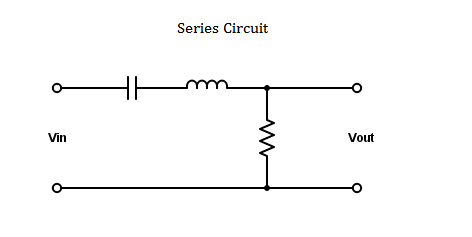
\includegraphics{SeriesCir.png}
    \caption{Our series circuit without oscilloscope or signal generator pictured.}
    \label{fig:sercir}
\end{figure}

This is our arrangement of circuit elements for our notch circuit.

\begin{figure}[H]
    \centering
    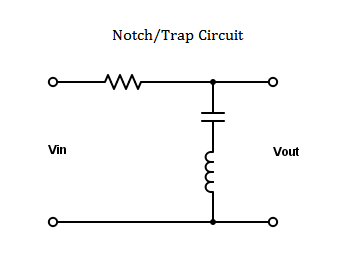
\includegraphics{NotchCir.png}
    \caption{Our notch/trap circuit.}
    \label{fig:trapcir}
\end{figure}

%=====================================================
%============ Importing pictures  ==========================
%=====================================================

% !! To be imported, all graphics must be converted !!
% !!    to encapsulated postscript (.eps format)    !!
% !!  The GNU Image Manipulation Program (GIMP) is  !!
% !!          capable of this conversion.           !!



\subsection{Data Collection}

In the first portion of the lab, we studied the behavior of the series RLC circuit. We measured the input and output voltages at various frequencies to find the transfer function. We then compared our data to the derived transfer function above.
$$T(\omega) = \frac{R}{\sqrt{R^2 + \omega^2L^2 + \frac{1}{\omega^2C^2}-\frac{2L}{C}}}$$

\begin{figure}[H]
    \centering
    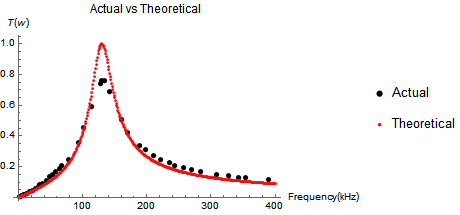
\includegraphics[scale = 0.8]{Series.png}
    \caption{Our series circuit data compared to the theoretical results.}
    \label{fig:sermodel}
\end{figure}

We can see from Figure \ref{fig:sermodel} that our data followed the theoretical model though we did not reach the 1 ratio for the transfer function. However the peak of the transfer function occurs at approximately 130 kHz based on the graph and 128 kHz based on the raw data. This is very close to our calculated resonance frequency of 129.95 kHz. We likely didn't reach the peak due to the internal impedance of the generator and oscilloscope.
We then found the phase shifts at resonance frequency and twice the resonance frequency.

\begin{figure}[H]
    \centering
    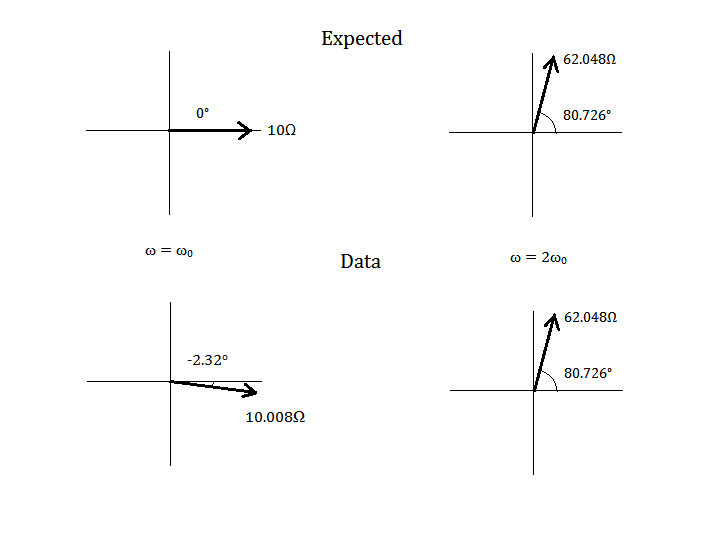
\includegraphics[scale = 0.8]{Phasor.png}
    \caption{Phasor diagrams for the resonance frequency $\omega_0$ and twice the resonance frequency $2\omega_0$.}
    \label{fig:phasor}
\end{figure}

The magnitude of our phase diagrams from our data was nearly exact for both frequencies however the phase shift at resonance frequency is not the same as what is expected. This may be due to some error in the oscilloscope finding the phase shift.

The power dissipated can be found using 

$$V=IR \text{ and } P = IV$$

Given a 10 rms-volts at resonance frequency, we find the current with $I=\frac{V}{Z}$ where Z is the total impedence. This gives a current of 1 Amps. Using $P=I_{rms}^2R$, we find that the power is 10 J. In order to find the power using the phase shift we must use
$$P = V_{rms}I_{rms}\cos(\phi)$$
In order to find the phase shift we use
$$\phi=\tan^{-1}\left(\frac{Z_L-Z_C}{R}\right)$$
At resonance frequency, we see that $\phi=0$ and $\cos(0) = 1$. Thus our power using phase shift is again 10 J.

Finally, we also studied and compared the behavior of the transfer function of the trap circuit. 

\begin{figure}[H]
    \centering
    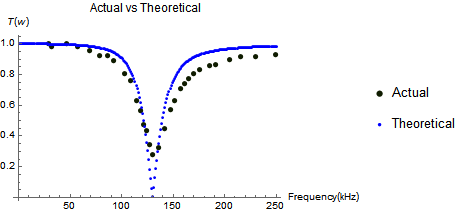
\includegraphics[scale = 0.8]{Notch.png}
    \caption{Our trap circuit data compared to the theoretical results.}
    \label{fig:trapmodel}
\end{figure}

We can see from Figure \ref{fig:trapmodel} that our data followed the theoretical model though as the series circuit it did not approach the lowest point. However the peak of the transfer function occurs at approximately 130 kHz based on the graph and raw data. This is also very close to our calculated resonance frequency of 129.95 kHz.

\section{Summary and conclusions}

We studied the behavior of RLC circuits. We found that the resonance frequency for out circuit was 129.96 kHz. We were able to accurately model the behavior of the transfer function of both configuration to their theoretical models. The calculated phase diagrams at resonance and two times the resonance were relatively close to the expected diagrams. The hypothetical power of a 10 rms-volt signal at resonance was found to be 10 J. 


%=====================================================
%============ Bibliography  ==============================
%=====================================================



%=====================================================
%============ End ====================================
%=====================================================

\end{document}

%=====================================================
%============ End ====================================
%=====================================================